\documentclass{article}
\usepackage{arxiv}

\usepackage[utf8]{inputenc}
\usepackage[english, russian]{babel}
\usepackage[T1]{fontenc}
\usepackage{url}
\usepackage{booktabs}
\usepackage{amsfonts}
\usepackage{nicefrac}
\usepackage{microtype}
\usepackage{lipsum}
\usepackage{graphicx}
\usepackage{natbib}
\usepackage{doi}



\title{A template for the \emph{arxiv} style}

\author{  Дмитрий Сергеевич Прокудин \\
	Факультет ВМК \\
    МГУ имени М.В.Ломоносова \\
	Москва, Россия \\
	\texttt{TheLoyalist@yandex.ru} \\
	%% examples of more authors
	\And
	Мой научник \\
	Факультет ВМК \\
    МГУ имени М.В.Ломоносова \\
	Москва, Россия \\
	\texttt{почтамоегонаучника@gmail.ru}  \\
	%% \AND
	%% Coauthor \\
	%% Affiliation \\
	%% Address \\
	%% \texttt{email} \\
	%% \And
	%% Coauthor \\
	%% Affiliation \\
	%% Address \\
	%% \texttt{email} \\
	%% \And
	%% Coauthor \\
	%% Affiliation \\
	%% Address \\
	%% \texttt{email} \\
}
\date{}

\renewcommand{\shorttitle}{\textit{arXiv} Template}

%%% Add PDF metadata to help others organize their library
%%% Once the PDF is generated, you can check the metadata with
%%% $ pdfinfo template.pdf
\hypersetup{
pdftitle={A template for the arxiv style},
pdfsubject={q-bio.NC, q-bio.QM},
pdfauthor={David S.~Hippocampus, Elias D.~Striatum},
pdfkeywords={First keyword, Second keyword, More},
}

\begin{document}
\maketitle

\begin{abstract}
Задача обнаружения аномалий в многомерных временных рядах является актуальной во многих областях, например, в производстве и технологических процессах, где аномальные значения могут указывать на неисправности в системе. Данные могут быть взаимосвязаны друг с другом и иметь сложную структуру, поэтому нейронные сети хорошо подходят для решения данной задачи.  
    
В данной работе сравниваются модели со сложными архитектурами, предназначенными конкретно для прогнозирования многомерных временных рядов, такие как Autoformer и TimesNet, и модели с более простыми архитектурами, предназначенными для работы с последовательностями в общем, такие как рекуррентные нейронные сети и временные свёрточные нейронные сети. Проводится экспериментальное исследование качества прогноза и обнаружения аномалий данными моделями. Рассматривается два метода обнаружения аномалий: на основе разности предсказанных значений и значений исходного ряда и на основе вероятностного подхода. Эксперименты подтверждают применимость рассмотренных моделей и методов для решения данной задачи и показывают преимущество временных свёрточных сетей над специализированными моделями - при более простой архитектуре точность прогноза оказывается выше. 
\end{abstract}


\keywords{Нейронные сети \and многомерные временные ряды \and обнаружение аномалий}

\section{Введение}
Задача обнаружения аномалий во временных рядах нередко возникает при эксплуатации сложных технологических систем. Их работа описывается множеством величин, изменяющихся во времени. Например, это могут быть показания сенсоров и датчиков или состояния различных устройств во время выполнения процесса. Во время нормальной работы эти значения чаще всего ведут себя регулярным образом с характерными значениями или периодичностью. Аномалией в таких данных является отклонение от типичного поведения. Необходимо уметь выявлять такие участки, так как они могут свидетельствовать о наличии сбоев или неисправностей в системе. Обычно части системы взаимосвязаны, поэтому сбой в одной из них может привести к серии сбоев и в других частях. Более того, даже незначительные отклонения от нормальной работы могут привести к существенным неисправностям через достаточно большой промежуток времени. Такая специфика задачи позволяет использовать нейронные сети для её решения, поскольку они способны обрабатывать большие объёмы данных и определять сложные и долговременные связи между компонентами системы. 

В данной работе применяются модели глубокого обучения для прогнозирования временных рядов и рассматриваются методы обнаружения аномалий на основе их прогноза. Проводится два эксперимента: в первом эксперименте на наборе данных MNIST сравниваются рекуррентные нейронные сети и временные свёрточные сети, и выбирается лучшая архитектура для дальнейшего анализа, во втором эксперименте непосредственно решается задача обнаружения аномалий на примере набора данных SWaT с применением временных свёрточных сетей, модели Autoformer и модели TimesNet.
\section{Постановка задачи}
\label{sec:headings}

Имеется многомерный временной ряд $X = \{x_1, x_2, x_3, ..., x_T\}, x_t \in R^k$, $k$ - количество каналов в ряду. Необходимо реализовать алгоритм $F$, оценивающий аномальность элемента $x_t$ исходного ряда: $F(x_t, X) = y_t, y_t \in R^m$. В общем случае, размерность $m$ оценки может отличаться от размерности $k$ ряда, например, при оценке аномальности только подвыборки каналов по значениям всех каналов. В данной работе $m$ принимается равным $k$. 

\subsection{Рассматриваемые архитектуры нейронных сетей}
В данной работе рассматривается и сравнивается два класса нейронных сетей:
\begin{enumerate}
\item Архитектуры, предназначенные для работы с последовательностями. 

Модели данной группы можно применять не только для прогнозирования временных рядов, но и для решения других задач, связанных с обработкой последовательностей. Среди моделей данной группы для данной работы были выбраны рекурретные и временные свёрточные нейронные сети. 

\item Архитектуры, предназначенные для работы только со временными рядами. 

Модели данной группы являются специализированными и предназначены конкретно для прогнозирования временных рядов. Для данной работы были выбраны Autoformer и TimesNet.
\end{enumerate}
\subsubsection{Рекуррентные нейронные сети}

Рекуррентные сети хорошо зарекомендовали себя для работы с последовательностями произвольной длины, включая временные ряды. В данной работе исследуются наиболее распространённые архитектуры: LSTM и GRU.

\subsection{Временные свёрточные сети}
Временная свёрточная сеть (Temporal Convolutional Network, далее TCN) была предложена как альтернатива рекуррентным сетям. В основе TCN лежит операция одномерной расширенной (dilated) временной (чтобы исключить 'заглядывание в будущее') свёртки: 

$F(s) = (x \ast_d f)(s) = \sum_{i=0}^{k - 1}f(i) \cdot x_{s - d \cdot i},$ для входа $(x_0, ..., x_T).$

$k$ - размер ядра свёртки, $d$ - 'фактор' расширения.

Расширенная свёртка позволяет увеличить поле восприятия TCN, параметр d экспоненциально увеличивается от слоя к слою.

\subsubsection{Autoformer}
По аналогии с рекуррентными сетями трансформеры предназначены для работы с последовательностями. Чтобы позволить трансформерам лучше справляться с долговременными зависимостями во временных рядах, в была предложена модель Autoformer. В ней используется идея отдельной работы с сезонной и трендовой компонентами временного ряда, а классический механизм внимания заменяется на механизм авто-корреляции, позволяющий находить зависимости между текущим значением и предыдущими значениями величины.

\subsubsection{TimesNet}
Для работы со временными рядами в было предложено обрабатывать временные ряды не в одномерном пространстве, а в двумерном, преобразовывая их на основе периодичности. Таким образом, можно обрабатывать внутри- и межпериодные вариации соответственно в строках и столбцах двумерных тензоров, используя для этого двумерные свёртки. Для реализации этой идеи была предложена рассматриваемая модель TimesNet.


\subsubsection{Headings: third level}
\lipsum[6]

\paragraph{Paragraph}
\lipsum[7]



\section{Examples of citations, figures, tables, references}
\label{sec:others}

\subsection{Citations}
Citations use \verb+natbib+. The documentation may be found at
\begin{center}
	\url{http://mirrors.ctan.org/macros/latex/contrib/natbib/natnotes.pdf}
\end{center}

Here is an example usage of the two main commands (\verb+citet+ and \verb+citep+): Some people thought a thing \citep{kour2014real, hadash2018estimate} but other people thought something else \citep{kour2014fast}. Many people have speculated that if we knew exactly why \citet{kour2014fast} thought this\dots

\subsection{Figures}
\lipsum[10]
See Figure \ref{fig:fig1}. Here is how you add footnotes. \footnote{Sample of the first footnote.}
\lipsum[11]

\begin{figure}
	\centering
	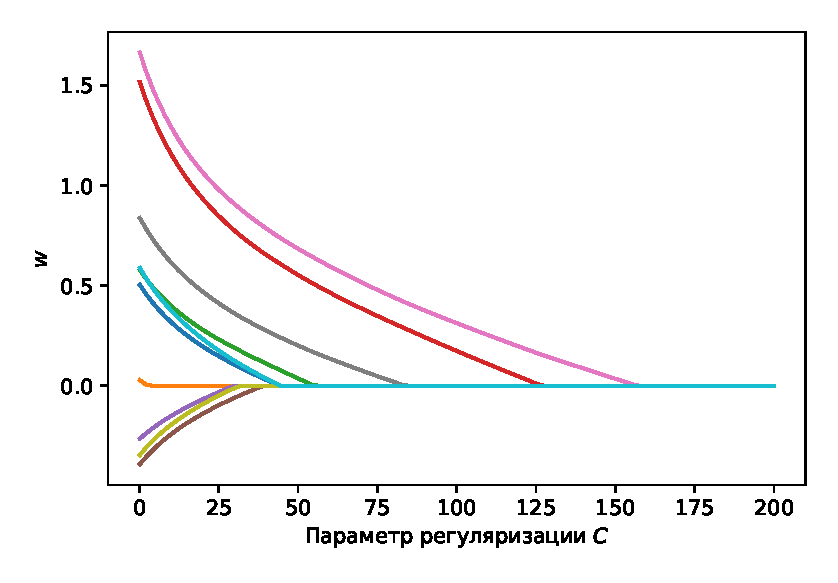
\includegraphics[width=0.5\textwidth]{../figures/log_reg_cs_exp.eps}
	\caption{Sample figure caption.}
	\label{fig:fig1}
\end{figure}

\subsection{Tables}
See awesome Table~\ref{tab:table}.

The documentation for \verb+booktabs+ (`Publication quality tables in LaTeX') is available from:
\begin{center}
	\url{https://www.ctan.org/pkg/booktabs}
\end{center}


\begin{table}
	\caption{Sample table title}
	\centering
	\begin{tabular}{lll}
		\toprule
		\multicolumn{2}{c}{Part}                   \\
		\cmidrule(r){1-2}
		Name     & Description     & Size ($\mu$m) \\
		\midrule
		Dendrite & Input terminal  & $\sim$100     \\
		Axon     & Output terminal & $\sim$10      \\
		Soma     & Cell body       & up to $10^6$  \\
		\bottomrule
	\end{tabular}
	\label{tab:table}
\end{table}

\subsection{Lists}
\begin{itemize}
	\item Lorem ipsum dolor sit amet
	\item consectetur adipiscing elit.
	\item Aliquam dignissim blandit est, in dictum tortor gravida eget. In ac rutrum magna.
\end{itemize}


\bibliographystyle{unsrtnat}
\bibliography{references}

\end{document}